%! Author = user
%! Date = 3/9/2024

% Preamble
\documentclass{article}
\usepackage[utf8]{inputenc}
\usepackage{amsmath, amssymb, amsthm}
\usepackage{tikz}
\usepackage{pgfplots}
\usepackage{subfigure}
\usepackage{listings}
\usepackage[fontsize=14pt]{fontsize}
\usepackage[a4paper,
            bindingoffset=.2in,
            left=.7in,
            right=.7in,
            top=1in,
            bottom=1in,
            footskip=.25in]{geometry}

\definecolor{dkgreen}{rgb}{0,0.6,0}
\definecolor{gray}{rgb}{0.5,0.5,0.5}
\definecolor{mauve}{rgb}{0.58,0,0.82}

\lstset{frame=tb,
  language=Java,
  aboveskip=3mm,
  belowskip=3mm,
  showstringspaces=false,
  columns=flexible,
  basicstyle={\small\ttfamily},
  numbers=none,
  numberstyle=\tiny\color{gray},
  keywordstyle=\color{blue},
  commentstyle=\color{dkgreen},
  stringstyle=\color{mauve},
  breaklines=true,
  breakatwhitespace=true,
  tabsize=3
}

\title{LaTex for Students}
\author{Jun Ho Lee}
\date{March 2024}

% Document
\begin{document}

\newpage

\section{Week1}

    Introduction to Deep Learning.

\subsection{What is a Neural Network?}

In machine learning, a neural network (also artificial neural network or neural net, abbreviated ANN or NN) is a model inspired by the neuronal organization found in the biological neural networks in animal brains. (from wikipedia)\\

An artificial neural network is an interconnected group of nodes, inspired by a simplification of neurons in a brain. Here, each circular node represents an artificial neuron and an arrow represents a connection from the output of one artificial neuron to the input of another.\\

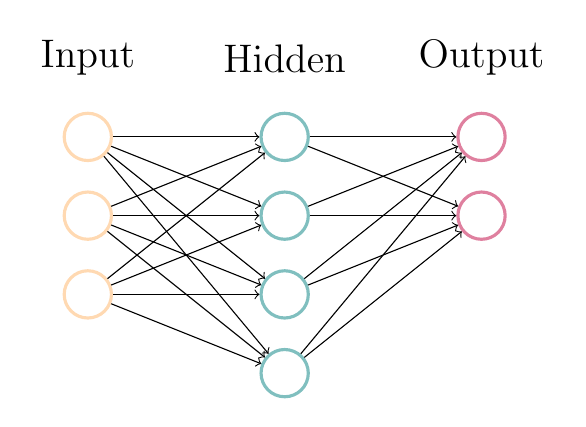
\begin{tikzpicture}
    % Input Layer
    \foreach \i in {1,2,3} {
        \node[circle, minimum size = 6mm, draw=orange!30, line width=.4mm] (Input-\i) at (0,-\i) {};
        \ifnum \i=1
            \node[above of=Input-\i] {Input};
        \fi
    }
    % Hidden Layer
    \foreach \i in {1,2,3,4} {
        \node[circle, minimum size = 6mm, draw=teal!50, line width=.4mm] (Hidden-\i) at (2.5,-\i) {};
        \ifnum \i=1
        \node[above of=Hidden-\i] {Hidden};
        \fi
    }
    % Output Layer
    \foreach \i in {1,2} {
        \node[circle, minimum size = 6mm, draw=purple!50, line width=.4mm] (Output-\i) at (5,-\i) {};
        \ifnum \i=1
        \node[above of=Output-\i] {Output};
        \fi
    }
    % Arrows
    \foreach \i in {1,2,3} {
        \foreach \j in {1,2,3,4} {
           \draw[->] (Input-\i) -- (Hidden-\j);
        }
    }
    \foreach \i in {1,2,3,4} {
        \foreach \j in {1,2} {
            \draw[->] (Hidden-\i) -- (Output-\j);
        }
    }
\end{tikzpicture}\\




\subsection{Supervised Learning with Neural Networks}


Standard NN, Convolutional NN, Recurrent NN.

\noindent Structured Data vs. Unstructured Data.

\subsection{Why is Deep Learning taking off?}

Scale drives deep learning progress.

\subsection{About this Course}
    \begin{enumerate}
        \item Neural Networks and Deep Learning
        \item Improving Deep Neural Networks: Hyperparameter  tuning, Regularization and Optimization
        \item Structuring your Machine Learning project
        \item Convolutional NeuralNetworks
        \item Natural Language Processing: Building sequence models
    \end{enumerate}

\subsection{Outline of this Course}
    \begin{itemize}
        \item{Week1. Introduction}
        \item{Week2. Basics of Neural Network programming}
        \item{Week3. One hidden layer Neural Networks}
        \item{Week4. Deep Neural Networks}
    \end{itemize}


\newpage
\section{Week2}

    Basics of Neural Network Programming

    How do I write an equation in \LaTeX?\\

    \begin{center}
    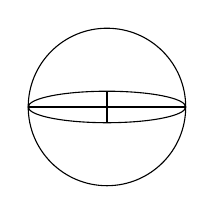
\begin{tikzpicture}
        \centering
        \draw (0,0) ellipse (1cm and 0.2cm);
        \draw (0,0) circle (1cm);
        \draw (0,-0.2) -- (0,0.2);
        \draw (-1,0) -- (1,0);
    \end{tikzpicture}
    \end{center}

    In 1902, Einstein created this equation: $E=mc^2$

    And Newton came up with this one: $\sum F=ma$

    \begin{equation}
        5+5=10
    \end{equation}

    \begin{equation}
        \begin{split}
            A & = \frac{5\pi r^2}{2} \\
            A & = \frac{1}{2} \pi r^2
        \end{split}
    \end{equation}

\newpage
\subsection{Neural Network Notations}

    \textbf{General comments:}\\
    superscript $(i)$ will denote the $i^{th}$ training example. \\
    superscript $[l]$ will denote the $l^{th}$ layer.\\

    \textbf{Sizes:}
    \begin{itemize}
        \item[-]{m: number of examples in the dataset}
        \item[-]{$n_x$: input size}
        \item[-]{$n_y$: output size}
        \item[-]{$n_h^{[l]}$: number of hidden units of the ${l^th}$ layer. \\ In a for loop, it is possible to denote $n_x = n_h^{[0]}$ and $n_y = n_h^{[number of layer+1]}$ }
        \item[-]{$L$: number of layers in the network}
    \end{itemize}

    \textbf{Objects:}
    \begin{itemize}
        \item[-]{$X \in \mathbb{R}^{n_x \times m}$ is the input matrix}
        \item[-]{$x^{(i)} \in \mathbb{R}^{n_x}$ is the $i^{th}$ example represented as a column vector }
        \item[-]{$Y \in \mathbb{R}^{n_y \times m}$ is the label matrix}
        \item[-]{$y^{(i)} \in \mathbb{R}^{n_y}$ is the output label for the $i^{th}$ example}
        \item[-]{$W^{[l]} \in \mathbb{R}\textsuperscript{$\sharp$ of units in next layer $\times$ $\sharp$ of units in the previous layer}$ is the weight matrix, superscript $[l]$ indicates the layer}
        \item[-]{}
    \end{itemize}

    \textbf{Common forward propagation equation examples:}
    \begin{itemize}
        \item[-]{}
        \item[-]{}
    \end{itemize}

    \textbf{Examples of cost functions:}
    \begin{itemize}
        \item[-]{}
        \item[-]{}
    \end{itemize}

\newpage
\subsection{Binary Classification}

    Use matrix without using for loops.\\
    Computation using Forward propagation and Backward propagation.\\
    Logistic regression is an algorithm for binary classification.\\

    m training examples
    $\{(X^{(1)}, Y^{(1)}), (X^{(2)}, Y^{(2)}), \hdots, (X^{(m)}, Y^{(m)})\}$ \\
    where $X^{(i)} \in \mathbb{R}^{n_x}$ and $Y^{(i)} \in \{0,1\}$ for $i \in [1,m]$ \\

    $X =
    \begin{bmatrix}
        \vdots & \vdots & \vdots & \vdots\\
        X^{(1)} & X^{(2)} & \dots & X^{(m)} \\
        \vdots & \vdots & \vdots & \vdots\\
    \end{bmatrix}
    \in \mathbb{R}^{n_x \times m}
    $\\

    $X.shape = (n_x, m)$\\

    $Y = [Y^{(1)}, Y^{(2)}, \hdots, Y^{(m)}]
    \in \mathbb{R}^{1 \times m}
    $\\

    $Y.shape = (1, m)$\\

\newpage
\subsection{Logistic Regression}

    Given $x$, want $\hat{y} = P(y=1 |x)$ where $x \in \mathbb{R}^{n_x}$\\

    Parameters: $w \in \mathbb{R}^{n_x}$ a $n_x$ dimensional vector, $b \in \mathbb{R}$ a real number.\\

    Output $\hat{y} = \sigma(w^{T}x + b) = \sigma(z)$\\

    $\displaystyle \sigma (z)=\frac {1}{1+e^{-z}}$\\

    Drawing a sigmoid function and its derivative in tikz\\

    \pgfplotsset{compat=1.16}
    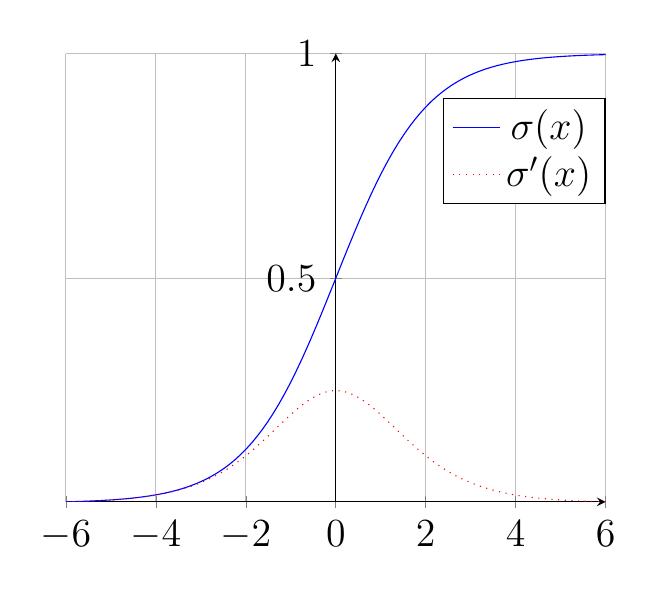
\begin{tikzpicture}[declare function={sigma(\x)=1/(1+exp(-\x));
    sigmap(\x)=sigma(\x)*(1-sigma(\x));}]
    \begin{axis}%
    [
        grid=major,
        xmin=-6,
        xmax=6,
        axis x line=bottom,
        ytick={0,.5,1},
        ymax=1,
        axis y line=middle,
        samples=100,
        domain=-6:6,
        legend style={at={(1,0.9)}}
    ]
        \addplot[blue,mark=none]   (x,{sigma(x)});
        \addplot[red,dotted,mark=none]   (x,{sigmap(x)});
        \legend{$\sigma(x)$,$\sigma'(x)$}
    \end{axis}
    \end{tikzpicture}


\newpage
\subsection{Logistic Regression Cost Function}

    To train the parameter $w$ and $b$ of a Logistic Regression Model, we need a cost function.\\

    $\hat{y} = \sigma{(w^{T}X + b)}$ where $\sigma(z) = \frac{1}{1+e^{-z}}$\\

    $\hat{y}^{(i)} = \sigma{(w^{T}X^{(i)} + b)}$ where $\sigma(z^{(i)}) = \frac{1}{1+e^{{-z}^{(i)}}}$\\

    Given $\{(x^{(1)}, y^{(1)}), (x^{(2)}, y^{(2)}), \hdots, (x^{(m)}, y^{(m)})\}$, want $\hat{y}^{(i)} \approx y^{(i)}$. \\

    Loss(error) function (for a single training Example):

    $\displaystyle \mathcal{L}(\hat{y}, y) = -(y\log{\hat{y}} + (1-y)\log{(1-\hat{y}))}$\\

    Cost function (for the entire training Examples):

    $\displaystyle \mathcal{J}(w, b) = \frac{1}{m}\sum_{i=1}^{m} \mathcal{L}(\hat{y}^{(i)}, y^{(i)}) = -\frac{1}{m}\sum_{i=1}^{m} [y^{(i)}\log{\hat{y}^{(i)}} + (1-y^{(i)})\log{(1-\hat{y}^{(i)})}]$\\\\

    The loss function computes the error for a single training example; the cost function is the average of the loss functions of the entire training set.\\

    In training logistic regression model, we will try to find $w$ and $b$ such that they minimize the Cost function $\mathcal{J}(w, b)$.\\

    Logistic Regression can be seen as a very small Neural Network.\\


\newpage
\subsection{Gradient Descent}

    $\displaystyle \mathcal{J}(w, b) = \frac{1}{m}\sum_{i=1}^{m} \mathcal{L}(\hat{y}^{(i)}, y^{(i)}) = -\frac{1}{m}\sum_{i=1}^{m} [y^{(i)}\log{\hat{y}^{(i)}} + (1-y^{(i)})\log{(1-\hat{y}^{(i)})}]$\\\\

    Want to find $w$ and $b$ that minimize the Cost function $\mathcal{J}(w,b)$.

    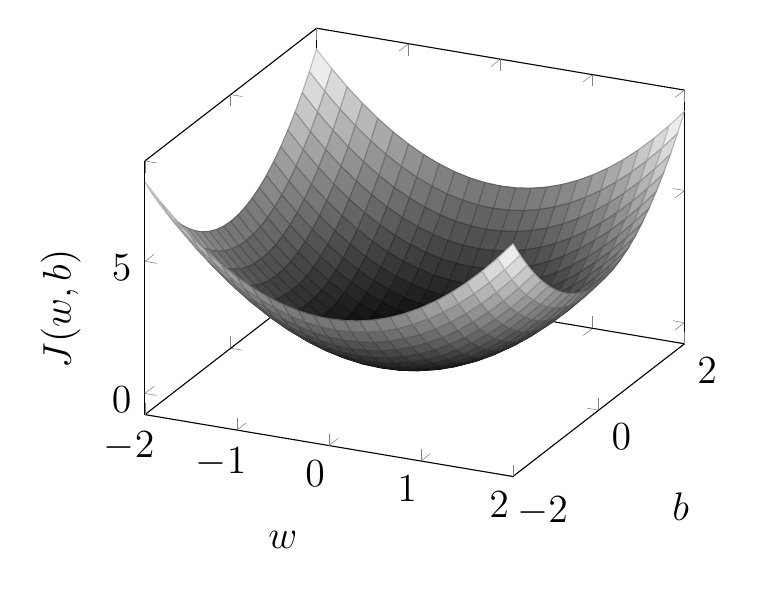
\begin{tikzpicture}
    \begin{axis}[
        xlabel=$w$,
        ylabel=$b$,
        zlabel={$J(w,b)$}
    ]
    \addplot3[surf,domain=-2:2, colormap/blackwhite] {x^2+y^2};
    \end{axis}
    \end{tikzpicture}\\

    $\mathcal{J}(w,b)$ is a convex function with a single local optimum.\\
    No matter where you initialize the point, you should get to the same point (Global optimum).\\

    Repeat: \\

        $w := w - \alpha \frac{\partial\mathcal{J}(w,b)}{\partial w} = w - \alpha dw$\\

        $b := b - \alpha \frac{\partial\mathcal{J}(w,b)}{\partial b} = b - \alpha db$\\

        where $\alpha$ is the learning rate.\\


\newpage
\subsection{Derivatives}

    derivatives; slope

    Given $f(a) = 3a$

    $\epsilon = .001, a= 2+\epsilon$

    $\frac{f(a)-f(a+\epsilon)}{\epsilon}$

    make $\epsilon$ close to zero $\rightarrow$ derivatives.

    $\frac{df(a)}{da} = \frac{d}{da} f(a)$

\subsection{More Derivative Examples}

    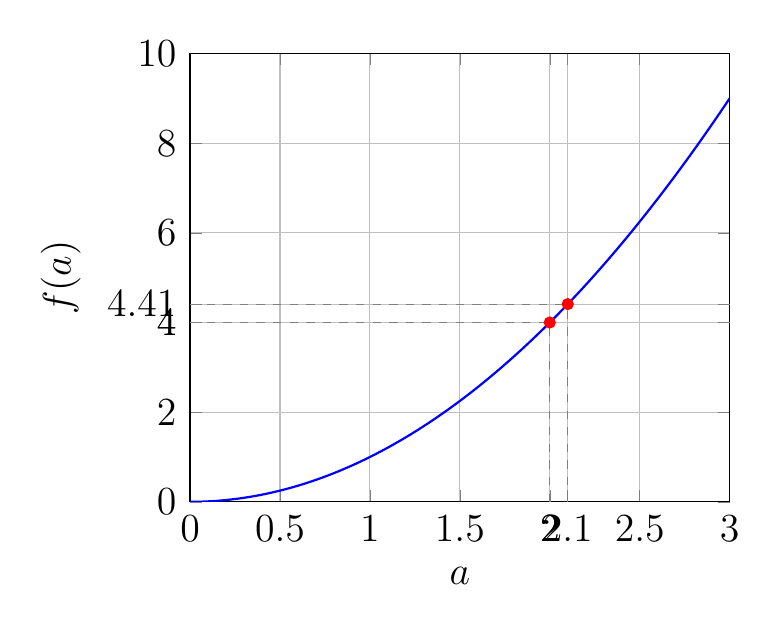
\begin{tikzpicture}
    \begin{axis}[
        xlabel=$a$,
        ylabel={$f(a)$},
        xmin=0, xmax=3,
        ymin=0, ymax=10,
        extra y ticks={4,4.41},
        extra y tick labels={$4$,$4.41$},
        extra x ticks={2,2.1},
        extra x tick labels={$2$,$2.1$},
        grid=major
    ]
    \addplot[domain=0:3, samples=100, thick, blue] {x^2};
    \addplot[only marks, red] coordinates {(2,4) (2.1,4.41)};
    \draw[dashed, gray] (axis cs:2,0) -- (axis cs:2,4);
    \draw[dashed, gray] (axis cs:0,4) -- (axis cs:2,4);
    \draw[dashed, gray] (axis cs:2.1,0) -- (axis cs:2.1,4.41);
    \draw[dashed, gray] (axis cs:0,4.41) -- (axis cs:2.1,4.41);
    \end{axis}
    \end{tikzpicture}

    $a=2$, $f(a)=4$\\

    $a=2.001$, $f(a)=4.004001$\\

    $\frac{d}{da}f(a) = 4$, when $a=2$\\

    $\frac{d}{da}f(a) = 10$, when $a=5$\\

    $\frac{d}{da}f(a) = \frac{d}{da}a^2 = 2a$\\

    Given a nudge $\epsilon= 0.001$ to $a$, the $f(a)$ goes up $2*a$.\\

\newpage
\subsection{Computation Graph}

    - Forward propagation step(forward pulse) : compute output of the network.\\
    - Backward pulse: compute the gradients or derivatives.

    $J(a,b,c) = 3(a+bc)$

    $u=bc$

    $v = a+u$

    $J=3v$

    In order to compute derivatices, you go backward propagation.

    One step of backward propagation on a computation graph yields derivative of final output variable.



\newpage
\subsection{Computing derivatives.}

    $u=bc$

    $v = a+u$

    $J=3v$

    Given $a=5, b=3, c=2$, then $v=11, J=33$

    We want to see how much $J$ changes if we change the values of $a,b,c,u,v$ for $J=3v$

    If we increase $v$ to 11.001, then $J=33.003$.

    $\frac{dJ}{dv} = 3$

    $a=5 \rightarrow a=5.001$

$v=11 \rightarrow a=11.001$

$J=33 \rightarrow a=33.003$\\

By Chain Rule:\\

$\frac{dJ}{da} = 3 = \frac{dJ}{dv}\frac{dv}{da} = 3 \times 1$\\

$\frac{dFinalOutputVar}{dvar}$ where $var$ can be $a,b,c,...$\\

We can simply denote $\frac{dJ}{dv} = dv$,
$\frac{dJ}{da} = da$, etc with respect to $J$.

Similarly, $\frac{dJ}{du} = \frac{dJ}{dv}\frac{dv}{du} = 3\times 1$

$\frac{dJ}{db} = \frac{dJ}{du}\frac{du}{db} = 3 \times 2 = 6$, where $u=bc = 2b$, and $\frac{du}{db} = 2$, given $a=5, b=3, c=2$.\\

$\frac{dJ}{dc} = \frac{dJ}{du}\frac{du}{dc} = 3 \times 3 = 9$, where $u=bc = 3c$, and $\frac{du}{dc} = 3$, given $a=5, b=3, c=2$.\\

$\displaystyle \frac{dJ}{da} = 3$\\

$\displaystyle \frac{dJ}{du} = 3$\\

$\displaystyle \frac{dJ}{db} = 6$\\

$\displaystyle \frac{dJ}{dc} = 9$\\

The coding convention $dvar$ represents:
The derivative of a final output variable with respect to various intermediate quantities.

\newpage
\subsection{Logistic Regression Gradient Descent}

On a single $i^{th}$ training example, $x^{(i)}$\\

Compute derivatives using Computation Graph(a bit overkill?) to implement/derive gradient descent for Logistic Regression.\\

Logistic regression recap:\\

$z^{(i)} = w^{T}x^{(i)} +b$\\

$\hat{y^{(i)}} = a^{(i)} = \sigma(z^{(i)})$\\

$\mathcal{L}(a^{(i)},y^{(i)}) = -(ylog(a^{(i)}) + (1-y^{(i)})log(1-a^{(i)}))$\\

Computation graph, given: $x_1$, $w_1$, $x_2$, $w_2$, $b$\\

% \fbox defaults text mode. Put '$' for math mode
$\fbox{$z^{(i)} = w_1 x_1 + w_2 x_2 +b$}$
$\rightarrow$
$\fbox{$\hat y^{(i)} = a^{(i)} = \sigma(z^{(i)})$}$
$\rightarrow$
$\fbox{$\mathcal{L}(a^{(i)},y^{(i)})$}$\\

, where $x^{(i)}= \begin{bmatrix}
x_1\\
x_2\\
\end{bmatrix}$\\

Modify $w$ and $b$ to reduce the loss $\mathcal{L}(a^{(i)},y^{(i)})$. In order to find such $w$ and $b$, we compute the derivatives with respect to $\mathcal{L}(a^{(i)},y^{(i)})$.\\

$\fbox{$da^{(i)}$}= \frac{d\mathcal{L}(a^{(i)},y^{(i)})}{da} = -\frac{d}{da} (y^{(i)}log(a^{(i)}) + (1-y^{(i)})log(1-a^{(i)})) = -\frac{y^{(i)}}{a^{(i)}} + \frac{1-y^{(i)}}{1-a^{(i)}}$\\

$\fbox{$dz^{(i)}$} = \frac{d\mathcal{L}(a^{(i)},y^{(i)})}{dz} = \frac{d\mathcal{L}(a^{(i)},y^{(i)})}{da} \frac{da}{dz} = (-\frac{y^{(i)}}{a^{(i)}}+\frac{1-y^{(i)}}{1-a^{(i)}})\frac{da}{dz}= a^{(i)}-y^{(i)}$

, where $\frac{da}{dz} = \frac{d}{dz}(\frac{1}{1+e^{-z^{(i)}}}) = \frac{e^{-z^{(i)}}}{(1+e^{-z^{(i)}})^2} = \frac{1}{1+e^{-z^{(i)}}}(1-\frac{1}{1+e^{-z^{(i)}}})= a^{(i)}(1-a^{(i)})$\\

\newpage

Go backward to compute :\\

$\fbox{$dw_1$} = \frac{\partial \mathcal{L}}{\partial w_1} =\frac{d\mathcal{L}(a,y)}{dw_1} =\frac{d\mathcal{L}(a,y)}{dz} \frac{dz}{dw_1}= x_1 dz$\\

$\fbox{$dw_2$} = \frac{\partial \mathcal{L}}{\partial w_2} =\frac{d\mathcal{L}(a,y)}{dw_2} =\frac{d\mathcal{L}(a,y)}{dz} \frac{dz}{dw_2}= x_2 dz$\\

$\fbox{db} = \frac{\partial \mathcal{L}}{\partial b} =\frac{d\mathcal{L}(a,y)}{db} =\frac{d\mathcal{L}(a,y)}{dz} \frac{dz}{db}= dz$\\\\

Compute $dz$ to compute $dw_1$, $dw_2$, $db$ and update with gradient descent:\\

$w_1 := w_1 - \alpha dw_1$\\

$w_2 := w_2 - \alpha dw_2$\\

$b := b - \alpha db $\\


\newpage
\subsection{Gradient Descent on $m$ Examples}

$\mathcal{J}(w,b) = \frac{1}{m}\sum_{i=1}^{m}\mathcal{L}(a^{(i)},y^{(i)})$\\

, where $a^{(i)} = \hat{y^{(i)}} = \sigma(z^{(i)}) = \sigma{(w^T x^{(i)} + b)}$\\

$\frac{\partial}{\partial w_1} \mathcal{J}(w,b) =\frac{1}{m}\sum_{i=1}^{m} \frac{\partial}{\partial w_1}\mathcal{L}(a^{(i)},y^{(i)})= \frac{1}{m}\sum_{i=1}^{m} dw_1^{(i)}$ \\

$\frac{\partial}{\partial w_2} \mathcal{J}(w,b) =\frac{1}{m}\sum_{i=1}^{m} \frac{\partial}{\partial w_2}\mathcal{L}(a^{(i)},y^{(i)})= \frac{1}{m}\sum_{i=1}^{m} dw_2^{(i)}$ \\

$\frac{\partial}{\partial b} \mathcal{J}(w,b) =\frac{1}{m}\sum_{i=1}^{m} \frac{\partial}{\partial b}\mathcal{L}(a^{(i)},y^{(i)})= \frac{1}{m}\sum_{i=1}^{m} db^{(i)}$ \\\\\\


Logistic regression on m examples:\\

$\noindent\fbox{%
\parbox{\textwidth}{%
$J=0$; $dw_1 = 0$; $dw_2 = 0$; $db=0$\\

for $i=1$ to $m$:\\
$\indent$ $z^{(i)} = w^T x^{(i)} + b$\\
$\indent$ $a^{(i)} = \sigma(z^{(i)})$\\
$\indent$ $\mathcal{J} += -[y^{(i)} log(a^{(i)}) + (1-y^{(i)})log(1-a^{(i)})]$\\
$\indent$ $dz^{(i)} = a^{(i)}- y^{(i)}$\\

* The value of $dw_1$, $dw_2$, $db$ in the code is cumulative:\\
$\indent$ $dw_1 += x_1^{(i)}dz^{(i)}$\\
$\indent$ $dw_2 += x_2^{(i)}dz^{(i)}$\\
$\dots$\\
$\indent$ $dw_{n_x} += x_{n_x}^{(i)}dz^{(i)}$\\

$\indent$ $db += dz^{(i)}$\\

$J/=m$,  $dw_1 /=m$,  $dw_2 /=m$,  $db /=m$\\
}%
}$\\

Finally, after finishing calculations for all m examples, we update(implment one step of gradient descent):\\

$w_1 := w_1 - \alpha dw_1$\\
$\indent w_2 := w_2 - \alpha dw_2$\\
$\indent \dots$ \\
$\indent w_{n_x} := w_{n_x} - \alpha dw_{n_x}$\\
$\indent b := b - \alpha db $\\

We have to do multiple steps of above gradient descent.\\

It has two weaknesses: two for-loops (one for m training examples and another for features: $w_{(i)}$ where $i$ can be big.) $\rightarrow$ $\fbox{Vectorization!}$

\newpage
\subsection{Vectorization}

What is vectorization?\\

$z = w^T+b$, where $w \in \mathcal{R}^{n_x}$ and $x \in \mathcal{R}^{n_x}$\\
\lstset{language=Python}
\begin{lstlisting}
import numpy as np

z = np.dot(w,x) + b
\end{lstlisting}


In Jupiter notebook:\\

\lstset{language=Python}
\begin{lstlisting}
import time

# 1. Vectorized version
a = np.random.rand(1000000)
b = np.random.rand(1000000)

tic = time.time()
c = np.dot(a,b)
toc = time.time()

print("1. Vectorized version:" + str(1000*(toc-tic))+ "ms")

# 2. For loop
c = 0
tic = time.time()
for i in range(1000000):
    c += a[i]*b[i]
toc = time.time()

print("2. For loop:" + str(1000*(toc-tic))+ "ms")
\end{lstlisting}

CPU and GPU has SIMD (single instruction multiple data). If you use built-in functions such as numpy's. It enables numpy to take better advantage of parallelization.

\newpage
\subsection{More Vectorization Examples}

Whenever possible, avoid explicit for-loops

$u = Av$\\
$u_i = \sum_{j}A_{ij}v_j$ for $i=1, \dots, n$\\

1. Non-vectorized:\\

\lstset{language=Python}
\begin{lstlisting}
import numpy as np

u = np.zeros((n,1))
for i in range(n):
    for j in range(m):
        u[i] += A[i][j]*v[j]
\end{lstlisting}

2. Vectorized:\\

\lstset{language=Python}
\begin{lstlisting}
import numpy as np

u = np.dot(A,v)
\end{lstlisting}

Vectors and matrix valued functions.\\
    say you need to apply the exponential operation on every element of a matrix/vector.

$v =
\begin{bmatrix}
v_1\\
\vdots\\
v_n\\
\end{bmatrix}
$\\

$u =
\begin{bmatrix}
e^{v_1}\\
\vdots\\
e^{v_n}\\
\end{bmatrix}
$\\

\lstset{language=Python}
\begin{lstlisting}
import numpy as np
u = np.zeros((n,1))

# 1. for-loop
for i in range(n):
    u[i] = math.exp(v[i])

# 2. Vectorized
u = np.exp(v)
u = np.log(v)
u = np.abs(v) # absolute value
u = np.maximum(v,0)
u = v**2
u = 1/v

\end{lstlisting}

Logistic regression derivatives\\

$\noindent\fbox{%
\parbox{\textwidth}{%
$J=0$; $dw_1 = 0$; $dw_2 = 0$; $db=0$\\

for $i=1$ to $m$:\\
$\indent$ $z^{(i)} = w^T x^{(i)} + b$\\
$\indent$ $a^{(i)} = \sigma(z^{(i)})$\\
$\indent$ $\mathcal{J} += -[y^{(i)} log(a^{(i)}) + (1-y^{(i)})log(1-a^{(i)})]$\\
$\indent$ $dz^{(i)} = a^{(i)}- y^{(i)}$\\

* The value of $dw_1$, $dw_2$, $db$ in the code is cumulative:\\
$\indent$ $dw_1 += x_1^{(i)}dz^{(i)}$\\
$\indent$ $dw_2 += x_2^{(i)}dz^{(i)}$\\
$\dots$\\
$\indent$ $dw_{n_x} += x_{n_x}^{(i)}dz^{(i)}$\\

$\indent$ $dw_2 += x_2^{(i)}dz^{(i)}$\\
$\indent$ $db += dz^{(i)}$\\

$J/=m$,  $dw_1 /=m$,  $dw_2 /=m$, \dots, $dw_{n_x} /=m$, $db /=m$\\

    }%
}$\\



\newpage
\subsection{Vectorizing Logistic Regression}

$z^{(i)} = w^T x^{(i)} + b$\\
$a^{(i)} = \sigma(z^{(i)})$ for $i=1, \dots, m$\\

$X =
\begin{bmatrix}
\vdots & \vdots & \dots & \vdots \\
x^{(1)} & x^{(2)} & \dots & x^{(m)}\\
\vdots & \vdots & \dots & \vdots \\
\end{bmatrix} \in \mathbb{R}^{n_x \times m}
$\\

$w \in \mathbb{R}^{n_x \times 1}$\\

$b =
\begin{bmatrix}
b & b & \dots & b\\
\end{bmatrix}
$\\

$Z =
w^T X +b =
\begin{bmatrix}
z^{(1)} & z^{(2)} & \dots & z^{(m)}\\
\end{bmatrix}
= \begin{bmatrix}
w^T x^{(1)} +b & w^T x^{(2)} +b & \dots & w^T x^{(m)} + b \\
\end{bmatrix}
$\\

, where $Z \in \mathbb{R}^{1 \times m}$\\

$A =
\begin{bmatrix}
a^{(1)} & a^{(2)} & \dots & a^{(m)}\\
\end{bmatrix}
=\begin{bmatrix}
\sigma(z^{(1)}) & \sigma(z^{(2)}) & \dots & \sigma(z^{(m)})\\
\end{bmatrix} = \sigma(Z)
$\\

\lstset{language=Python}
\begin{lstlisting}
import numpy as np

# Broadcasting: even though b is in 1xR, it spans as a vector
Z = np.dot(w.T, x) + b

\end{lstlisting}

\newpage
\subsection{Vectorizing Logistic Regression's Gradient Output}

$dz^{(i)} = a^{(i)}- y^{(i)}$\\
$dZ = \begin{bmatrix}
dz^{(1)}, & \dots & , dz^{(m)} \\
\end{bmatrix} $\\

$A = \begin{bmatrix}
a^{(1)}, & \dots & , a^{(m)} \\
\end{bmatrix} $\\

$Y = \begin{bmatrix}
y^{(1)}, & \dots & , y^{(m)} \\
\end{bmatrix} $\\

$dZ = A-Y =
\begin{bmatrix}
a^{(1)} - y^{(1)}, & \dots & , a^{(m)}-y^{(m)} \\
\end{bmatrix} $\\

$\noindent\fbox{%
\parbox{\textwidth}{%
$J=0$; $dw_1 = 0$; $dw_2 = 0$; $db=0$\\

\textcolor{blue}{for $i=1$ to $m$:}\\
$\indent$ $z^{(i)} = w^T x^{(i)} + b$\\
$\indent$ $a^{(i)} = \sigma(z^{(i)})$\\
$\indent$ $\mathcal{J} += -[y^{(i)} log(a^{(i)}) + (1-y^{(i)})log(1-a^{(i)})]$\\
$\indent$ $dz^{(i)} = a^{(i)}- y^{(i)}$\\

\textcolor{red}{* The value of $dw_1$, $dw_2$, $\dots$, $dw_{n_x}$, $db$ in the code is cumulative:}\\
$\indent$ $dw_1 += x_1^{(i)}dz^{(i)}$\\
$\indent$ $dw_2 += x_2^{(i)}dz^{(i)}$\\
$\dots$\\
$\indent$ $dw_{n_x} += x_{n_x}^{(i)}dz^{(i)}$\\

$\indent$ $db += dz^{(i)}$\\

$J/=m$,  $dw_1 /=m$,  $dw_2 /=m$, \dots, $dw_{n_x} /=m$, $db /=m$\\
    }%
}$\\


$db = \frac{1}{m}\sum_{i=1}^{m}dz^{(i)} = \frac{1}{m}$np.sum($dz$)\\

$dw = \frac{1}{m} X dz^{T} = \frac{1}{m} \begin{bmatrix}
x_1^{(1)} & x_1^{(2)} & \dots & x_1^{(m)}\\
x_2^{(1)} & x_2^{(2)} & \dots & x_2^{(m)}\\
\vdots & \vdots & \dots & \vdots \\
x_{n_x}^{(1)} & x_{n_x}^{(2)} & \dots & x_{n_x}^{(m)}\\
\end{bmatrix}
\begin{bmatrix}
dz^{(1)} \\
\vdots \\
dz^{(m)} \\
\end{bmatrix}\\
= \frac{1}{m} \begin{bmatrix}
\vdots & \vdots & \dots & \vdots \\
X^{(1)} & X^{(2)} & \dots & X^{(m)}\\
\vdots & \vdots & \dots & \vdots \\
\end{bmatrix}
\begin{bmatrix}
dz^{(1)} \\
\vdots \\
dz^{(m)} \\
\end{bmatrix}
= \frac{1}{m} \begin{bmatrix}
X^{(1)}dz^{(1)} + \dots + X^{(m)}dz^{(m)}\\
\end{bmatrix}
$\\


Vectorize:\\

$dw += x^{(i)}dz^{(i)}$\\

$Z = w^T + b = np.dot(w.T,X) + b$\\

$A = \sigma(Z)$\\

\textcolor{blue}{$dZ = A-Y$}\\

\textcolor{red}{$dw = \frac{1}{m} X dZ^T$}\\

$db = \frac{1}{m}$ np.sum($dZ$)\\

Single Iteration of Gradient Descent for Logistic Regression: \\

$w := w-\alpha dw$\

$b := b-\alpha db$\\

\newpage
\subsection{Broadcasting in Python}

Calories from Carbs, Proteins, Fats in 100g of different foods: \\

$\begin{bmatrix}
& Apples & Beef & Eggs & Potatoes \\
Carb & 56.0 & 0.0 & 4.4 & 68.0 \\
Protein & 1.2 & 104.0 & 52.0 & 8.0 \\
Fat & 1.8 & 135.0 & 99.0 & 0.9 \\
\end{bmatrix}$\\

Calculate the percentage of calories for Carb, Potein, Fat:\\

\lstset{language=Python}
\begin{lstlisting}
import numpy as np

A = np.array[[56.0, 0.0, 4.4, 68.0],
    [1.2, 104.0, 52.0, 8.0],
    [1.8, 135.0, 99.0, 0.9]])
print(A)

# sum vertically(axis=0)
cal = A.sum(axis=0)
print(cal)

# compute percentage
percentage = 100* A/cal.reshape(1,4)
print(percentage)
\end{lstlisting}


General Principle:\\

$(m,n)$ matrix operation $\rightarrow$ (1,n),(1,m) $\rightarrow$ (m,n), (m,n)\\

$(m,n)$ + real number $\mathbb{R}$ $\rightarrow$ (m+$\mathbb{R}$,n+$\mathbb{R}$)\\


\newpage
\subsection{}


\end{document}

